\documentclass[a4paper]{article}
\usepackage{vntex}
%\usepackage[english,vietnam]{babel}
%\usepackage[utf8]{inputenc}

%\usepackage[utf8]{inputenc}
%\usepackage[francais]{babel}
\usepackage{a4wide,amssymb,epsfig,latexsym,multicol,array,hhline,fancyhdr}
\usepackage{hyperref}
\usepackage{booktabs}
\usepackage{amsmath}
\usepackage{lastpage}
\usepackage[lined,boxed,commentsnumbered]{algorithm2e}
\usepackage{enumerate}
\usepackage{color}
\usepackage{graphicx}							% Standard graphics package
\usepackage{float} % Include the float package
\usepackage{array}
\usepackage{tabularx, caption}
\usepackage{multirow}
\usepackage[framemethod=tikz]{mdframed}% For highlighting paragraph backgrounds
\usepackage{multicol}
\usepackage{rotating}
\usepackage{graphics}
\usepackage{geometry}
\usepackage{setspace}
\usepackage{epsfig}
\usepackage{tikz}
\usepackage{listings}
\usetikzlibrary{arrows,snakes,backgrounds}
\usepackage{hyperref}
\hypersetup{urlcolor=blue,linkcolor=black,citecolor=black,colorlinks=true} 
%\usepackage{pstcol} 								% PSTricks with the standard color package

\newtheorem{theorem}{{\bf Định lý}}
\newtheorem{property}{{\bf Tính chất}}
\newtheorem{proposition}{{\bf Mệnh đề}}
\newtheorem{corollary}[proposition]{{\bf Hệ quả}}
\newtheorem{lemma}[proposition]{{\bf Bổ đề}}

\everymath{\color{blue}}
%\usepackage{fancyhdr}
\setlength{\headheight}{40pt}
\pagestyle{fancy}
\fancyhead{} % clear all header fields
\fancyhead[L]{
 \begin{tabular}{rl}
    \begin{picture}(25,15)(0,0)
    \put(0,-8){
\includegraphics[width=8mm, height=8mm]{logoITSGUsmall.png}}
    %\put(0,-8){\epsfig{width=10mm,figure=hcmut.eps}}
   \end{picture}&
	%\includegraphics[width=8mm, height=8mm]{hcmut.png} & %
	\begin{tabular}{l}
		\textbf{\bf \ttfamily Trường Đại học Sài Gòn}\\
		\textbf{\bf \ttfamily Khoa Công Nghệ Thông Tin}
	\end{tabular} 	
 \end{tabular}
}
\fancyhead[R]{
	\begin{tabular}{l}
		\tiny \bf \\
		\tiny \bf 
	\end{tabular}  }
\fancyfoot{} % clear all footer fields
\fancyfoot[L]{\scriptsize \ttfamily Bài tập lớn môn Phát triển phần mềm mã nguồn mở - Niên khóa 2023-2024}
\fancyfoot[R]{\scriptsize \ttfamily Trang {\thepage}/\pageref{LastPage}}
\renewcommand{\headrulewidth}{0.3pt}
\renewcommand{\footrulewidth}{0.3pt}


%%%
\setcounter{secnumdepth}{4}
\setcounter{tocdepth}{3}
\makeatletter
\newcounter {subsubsubsection}[subsubsection]
\renewcommand\thesubsubsubsection{\thesubsubsection .\@alph\c@subsubsubsection}
\newcommand\subsubsubsection{\@startsection{subsubsubsection}{4}{\z@}%
                                     {-3.25ex\@plus -1ex \@minus -.2ex}%
                                     {1.5ex \@plus .2ex}%
                                     {\normalfont\normalsize\bfseries}}
\newcommand*\l@subsubsubsection{\@dottedtocline{3}{10.0em}{4.1em}}
\newcommand*{\subsubsubsectionmark}[1]{}
\makeatother

\definecolor{dkgreen}{rgb}{0,0.6,0}
\definecolor{gray}{rgb}{0.5,0.5,0.5}
\definecolor{mauve}{rgb}{0.58,0,0.82}

\lstset{frame=tb,
	language=Matlab,
	aboveskip=3mm,
	belowskip=3mm,
	showstringspaces=false,
	columns=flexible,
	basicstyle={\small\ttfamily},
	numbers=none,
	numberstyle=\tiny\color{gray},
	keywordstyle=\color{blue},
	commentstyle=\color{dkgreen},
	stringstyle=\color{mauve},
	breaklines=true,
	breakatwhitespace=true,
	tabsize=3,
	numbers=left,
	stepnumber=1,
	numbersep=1pt,    
	firstnumber=1,
	numberfirstline=true
}

\begin{document}

\begin{titlepage}
\begin{center}
TRƯỜNG ĐẠI HỌC SÀI GÒN \\
KHOA CÔNG NGHỆ THÔNG TIN
\end{center}
\vspace{1cm}

\begin{figure}[h!]
\begin{center}

\includegraphics[width=3cm]{logoITSGU.png}
\end{center}
\end{figure}

\vspace{1cm}


\begin{center}
\begin{tabular}{c}
	\multicolumn{1}{l}{\textbf{{\Large PHÁT TRIỂN PHẦN MỀM MÃ NGUỒN MỞ}}}\\
	~~\\
	\hline
	\\
	\multicolumn{1}{l}{\textbf{{\Large Xây dựng phần mềm}}}\\
	\\
	
	\textbf{{\Huge Play Audio trên PYTHON}}\\
	\\
	\hline
\end{tabular}
\end{center}

\vspace{3cm}

\begin{table}[h]
\begin{tabular}{rrl}
\hspace{5 cm} & GVHD: &Từ Lãng Phiêu\\
& SV: & Phạm Hoàng Vũ - 3119560083\\
% & & SV3 - MSSV \\
% & & SV4 - MSSV\\
\end{tabular}
\vspace{1.5 cm}
\end{table}

\begin{center}

{\footnotesize TP. HỒ CHÍ MINH, THÁNG 2/2024}
\end{center}
\end{titlepage}


\thispagestyle{empty}

\newpage
\tableofcontents
\newpage

%%%%%%%%%%%%%%%%%%%%%%%%%%%%%%%%%


%%%%%%%%%%%%%%%%%%%%%%%%%%%%%%%%%
\section{Phần giới thiệu}
Kết quả của dự án là 1 phần mềm play audio, được thiết kế để cung cấp trải nghiệm nghe nhạc và âm thanh dễ dàng và tiện lợi. Phần mềm cho phép người dùng phát các tệp âm thanh mp3, quản lý danh sách phát, v.v. với một giao diện vô cùng thân thiện. Mục tiêu của dự án là mang đến một công cụ hữu ích cho việc thưởng thức âm nhạc hàng ngày. \\
Dự án được phát triển bằng ngôn ngữ Python cùng với các thư viện Tkinter, Pygame và trên môi trường Linux. 
\newpage
\section{Cơ sở lý thuyết}
\subsection{Giới thiệu thư viện Tkinter}

Tkinter là thư viện tiêu chuẩn của Python dùng để tạo giao diện đồ họa (GUI). Thư viện này cung cấp một tập hợp các widget (các thành phần giao diện như nút bấm, nhãn, hộp văn bản, v.v.) để xây dựng các ứng dụng GUI một cách dễ dàng và nhanh chóng.

Một số đặc điểm chính của thư viện Tkinter:

\begin{itemize}
    \item \textbf{Đơn giản và dễ sử dụng}: Tkinter được tích hợp sẵn trong Python, không cần cài đặt thêm các gói bổ sung. Cú pháp của Tkinter rất trực quan và dễ học, phù hợp cho người mới bắt đầu.
    \item \textbf{Đa nền tảng}: Các ứng dụng được xây dựng bằng Tkinter có thể chạy trên nhiều hệ điều hành khác nhau như Windows, macOS và Linux mà không cần thay đổi mã nguồn.
    \item \textbf{Hỗ trợ nhiều widget}: Tkinter cung cấp nhiều loại widget khác nhau như Button, Label, Entry, Text, Frame, Canvas, v.v., giúp lập trình viên dễ dàng thiết kế các giao diện phức tạp.
    \item \textbf{Khả năng mở rộng}: Tkinter cho phép lập trình viên mở rộng chức năng của các widget hiện có hoặc tạo các widget mới tùy theo nhu cầu.
\end{itemize}

Tkinter được sử dụng để thiết kế giao diện cho toàn bộ dự án này.

\subsection{Giới thiệu thư viện Pygame}

Pygame là một thư viện của Python, được sử dụng chủ yếu để phát triển trò chơi và các ứng dụng đa phương tiện. Tuy nhiên bên cạnh đó, ngoài khả năng xử lý đồ họa và sự kiện, Pygame còn cung cấp các công cụ mạnh mẽ để xử lý âm thanh, làm cho nó trở thành một lựa chọn tuyệt vời để xây dựng các ứng dụng phát âm thanh.

Một số tính năng chính của Pygame trong việc xây dựng ứng dụng âm thanh bao gồm:

\begin{itemize}
    \item \textbf{Phát và kiểm soát âm thanh}: Pygame hỗ trợ phát các tệp âm thanh ở nhiều định dạng khác nhau như WAV, MP3, và OGG. Người dùng có thể dễ dàng kiểm soát việc phát, tạm dừng, và dừng các bản nhạc hoặc hiệu ứng âm thanh.
    \item \textbf{Quản lý âm lượng}: Thư viện cho phép điều chỉnh âm lượng của các tệp âm thanh riêng lẻ hoặc toàn bộ âm thanh của ứng dụng, mang lại sự linh hoạt trong việc kiểm soát trải nghiệm nghe của người dùng.
    \item \textbf{Hỗ trợ đa kênh}: Pygame cung cấp khả năng phát nhiều tệp âm thanh đồng thời, hữu ích cho việc tạo ra các hiệu ứng âm thanh phong phú và đa dạng trong ứng dụng.
    \item \textbf{Dễ sử dụng và tích hợp}: Pygame có cú pháp đơn giản và dễ hiểu, giúp lập trình viên nhanh chóng nắm bắt và tích hợp vào ứng dụng của mình.
\end{itemize}

Ví dụ, dưới đây là mã Python đơn giản để phát một tệp âm thanh bằng Pygame: \\

Pygame không được tích hợp sẵn trong Python như Tkinter nên để sử dụng ta cần phải cài đặt
\begin{verbatim}
# Cài đặt Pygame bằng câu lệnh pip
pip install pygame
\end{verbatim}
\\
Code minh họa phát một tệp âm thanh bằng Pygame:
\begin{verbatim}
import pygame

# Khởi tạo Pygame
pygame.init()

# Tải và phát tệp âm thanh
pygame.mixer.music.load('path/to/your/audiofile.mp3')
pygame.mixer.music.play()

# Vòng lặp chính để giữ chương trình chạy
running = True
while running:
    for event in pygame.event.get():
        if event.type == pygame.QUIT:
            running = False

# Dừng phát âm thanh và thoát
pygame.mixer.music.stop()
pygame.quit()
\end{verbatim}

Với Pygame, việc xây dựng một ứng dụng phát âm thanh trở nên đơn giản và hiệu quả, mang lại trải nghiệm nghe tuyệt vời cho người dùng.

\newpage

\section{Thiết kế ứng dụng}
\subsection{Các tính năng của ứng dụng}
\subsubsection{Quản lí playlist}
Ứng dụng phát âm thanh không chỉ đơn thuần là một trình phát nhạc, mà còn tích hợp tính năng quản lý playlist mạnh mẽ, giúp người dùng dễ dàng quản lý và tuỳ chỉnh trải nghiệm nghe nhạc của mình. Các tính năng quản lý playlist bao gồm:

\begin{itemize}
    \item \textbf{Tìm kiếm Playlist}: Người dùng có thể dễ dàng tìm kiếm các playlist đã lưu của mình bằng cách nhập từ khóa. Tính năng tìm kiếm nhanh chóng và hiệu quả, giúp người dùng truy cập ngay lập tức vào playlist mong muốn.
    \item \textbf{Thêm Playlist}: Ứng dụng cho phép người dùng tạo và lưu nhiều playlist khác nhau. Người dùng có thể đặt tên cho playlist mới, thêm các tệp âm thanh yêu thích vào đó và sắp xếp theo thứ tự mong muốn.
    \item \textbf{Xóa Playlist}: Khi không cần thiết, người dùng có thể dễ dàng xóa các playlist không còn sử dụng. Tính năng này giúp người dùng quản lý không gian lưu trữ và giữ cho danh sách playlist luôn gọn gàng.
\end{itemize}

Với các tính năng này, ứng dụng không chỉ mang đến trải nghiệm nghe nhạc tuyệt vời mà còn cung cấp công cụ quản lý âm nhạc tiện lợi và hiệu quả. Người dùng có thể tạo các playlist phù hợp với tâm trạng hoặc hoạt động của mình, từ đó tối ưu hóa trải nghiệm nghe nhạc hàng ngày.
\subsubsection{Quản lí bài hát}
Ứng dụng phát âm thanh không chỉ cung cấp khả năng phát nhạc mà còn tích hợp các tính năng quản lý bài hát mạnh mẽ, giúp người dùng dễ dàng kiểm soát và tổ chức thư viện âm nhạc của mình. Các tính năng quản lý bài hát bao gồm:

\begin{itemize}
    \item \textbf{Tìm kiếm Bài hát}: Người dùng có thể nhanh chóng tìm kiếm các bài hát trong thư viện của mình bằng cách nhập tên bài hát. Tính năng tìm kiếm thông minh giúp người dùng dễ dàng truy cập ngay lập tức vào bài hát mong muốn.
    \item \textbf{Thêm Bài hát vào Playlist}: Ứng dụng cho phép người dùng thêm các bài hát yêu thích vào các playlist khác nhau. Điều này giúp người dùng tùy chỉnh các playlist theo ý thích và nhu cầu nghe nhạc của mình.
    \item \textbf{Xóa Bài hát khỏi Playlist}: Khi không còn nhu cầu, người dùng có thể dễ dàng xóa các bài hát khỏi playlist. Tính năng này giúp duy trì sự gọn gàng và tổ chức cho các playlist cá nhân.
\end{itemize}

Với các tính năng này, ứng dụng không chỉ mang đến trải nghiệm nghe nhạc tuyệt vời mà còn cung cấp các công cụ quản lý bài hát tiện lợi và hiệu quả. Người dùng có thể dễ dàng tìm kiếm, tổ chức và tùy chỉnh thư viện âm nhạc của mình, từ đó nâng cao trải nghiệm nghe nhạc hàng ngày.

\subsection{Cấu trúc mã nguồn}
\begin{figure}[H]
    \centering
    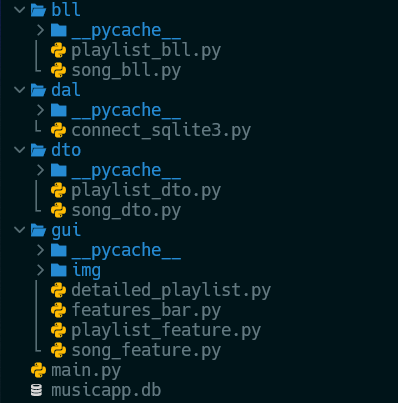
\includegraphics[width=0.5\textwidth]{file_structure.PNG}
    \caption{Cấu trúc các file}
    \label{fig:example_image}
\end{figure}

Ứng dụng được xây dựng theo kiến trúc mô hình ba lớp.
\begin{itemize}
    \item \textbf{GUI}: lớp tương tác trực tiếp với người dùng. Lớp này chịu trách nhiệm hiển thị và cung cấp các chức năng cần thiết để người dùng có thể tương tác với ứng dụng. Trong ứng dụng play audio này, GUI bao gồm các thành phần như cửa sổ chính, các nút điều khiển phát nhạc, và các biểu mẫu quản lý playlist và bài hát.
    \item \textbf{img}: chứa các file ảnh hỗ trợ tạo giao diện(không phải là thành phần chính của mô hình 3 lớp)
    \item \textbf{BLL}: lớp xử lý các logic nghiệp vụ của ứng dụng. Đây là nơi thực hiện các quy tắc, điều kiện và quy trình mà ứng dụng cần thực hiện. Trong ứng dụng này, BLL chịu trách nhiệm quản lý các thao tác liên quan đến playlist, như tìm kiếm, thêm, xóa playlist, cũng như quản lý các bài hát trong mỗi playlist.
    \item \textbf{DAL}: lớp chịu trách nhiệm truy cập và thao tác dữ liệu trong cơ sở dữ liệu. DAL bao gồm các phương thức để thực hiện các hoạt động như thêm, sửa, xóa và truy vấn dữ liệu từ cơ sở dữ liệu. Trong ứng dụng này, DAL quản lý việc lưu trữ thông tin về playlist và bài hát, đảm bảo rằng dữ liệu được lưu trữ một cách an toàn và hiệu quả.
    \item \textbf{DTO}: chứa các file vận chuyển dữ liệu giữa các lớp(không phải là thành phần chính của mô hình 3 lớp)
\end{itemize}


\section{Kết quả xây dựng}
\subsection{Mã nguồn}
\subsubsection{main.py}
Đây là file được dùng để khởi chạy toàn bộ dự án. 
\begin{mdframed}[hidealllines=true,backgroundcolor=magenta!10]
\begin{lstlisting}

from tkinter import *
from ttkbootstrap.constants import *
from gui.features_bar import FeaturesBar
import ttkbootstrap as tb


root = tb.Window(themename='darkly')

root.title('Music App')
root.geometry('500x500')

# features bar
featuresBar = FeaturesBar(root)
featuresBar.grid(row=0, column=0, sticky="nsew", padx=5)

root.mainloop()

\end{lstlisting}
\end{mdframed}


\begin{itemize}
    \item \texttt{from tkinter import *}: Nhập toàn bộ các module và hàm từ thư viện Tkinter, một thư viện chuẩn của Python dùng để tạo giao diện người dùng.
    \item \texttt{from ttkbootstrap.constants import *}: Nhập toàn bộ các hằng số từ thư viện ttkbootstrap, giúp tạo các giao diện người dùng với các chủ đề hiện đại.
    \item \texttt{from gui.features\_bar import FeaturesBar}: Nhập lớp \texttt{FeaturesBar} từ module \texttt{gui.features\_bar}, đây là một thành phần của giao diện người dùng trong ứng dụng.
    \item \texttt{import ttkbootstrap as tb}: Nhập thư viện ttkbootstrap và đặt tên viết tắt là \texttt{tb} để dễ dàng sử dụng.
    \item \texttt{root = tb.Window(themename='darkly')}: Dòng này tạo một cửa sổ chính cho ứng dụng với chủ đề "darkly" từ thư viện ttkbootstrap.
    \item \texttt{root.title('Music App')}: Đặt tiêu đề cho cửa sổ chính là "Music App".
    \item \texttt{root.geometry('500x500')}: Đặt kích thước cho cửa sổ chính là 500x500 pixel.
    \item \texttt{featuresBar = FeaturesBar(root)}: Tạo một đối tượng \texttt{FeaturesBar} và gắn nó vào cửa sổ chính \texttt{root}.
    \item \texttt{featuresBar.grid(row=0, column=0, sticky="nsew", padx=5)}: Đặt \texttt{featuresBar} vào lưới của cửa sổ chính tại hàng 0 và cột 0, với các tùy chọn "sticky" để mở rộng và "padx" để thêm khoảng cách ngang.
    \item \texttt{root.mainloop()}: Dòng này bắt đầu vòng lặp chính của giao diện người dùng, giữ cho cửa sổ mở và phản hồi các sự kiện từ người dùng cho đến khi cửa sổ bị đóng.
\end{itemize}

Tóm lại, đoạn mã này tạo ra một cửa sổ ứng dụng phát nhạc với một thanh tính năng (\texttt{FeaturesBar}) được đặt trong lưới (\texttt{grid}) của cửa sổ chính. Cửa sổ sử dụng chủ đề "darkly" từ ttkbootstrap để có giao diện hiện đại và bắt mắt.


\subsubsection{features\_bar.py}
File này tạo giao diện thanh chức năng của ứng dụng. Cho phép người dùng lựa chọn sử dụng các chức năng của ứng dụng.
\begin{mdframed}[hidealllines=true,backgroundcolor=magenta!10]
\begin{lstlisting}

from tkinter import *
from PIL import Image, ImageTk
from .playlist_feature import PlaylistFeature_Frame
from .song_feature import SongFeature_Frame
from ttkbootstrap.constants import *
import ttkbootstrap as tb

class FeaturesBar(tb.Frame):
    def __init__(self, master):
        self.master = master
        super().__init__(self.master)

        # Icons (assuming these are pre-loaded elsewhere)
        self.icon_images = {
            "home": ImageTk.PhotoImage(Image.open('./gui/img/home.png')),
            "playlists": ImageTk.PhotoImage(Image.open('./gui/img/playlist.png')),
        }
        self.icon_on_images = {
            "home": ImageTk.PhotoImage(Image.open('./gui/img/home_on.png')),
            "playlists": ImageTk.PhotoImage(Image.open('./gui/img/playlist_on.png')),
        }

        # Create icon labels
        self.icon_labels = {}  # Dictionary to store label references
        for icon_name, image in self.icon_images.items():
            label = tb.Label(self, image=image)
            label.bind("<Enter>", self.on_enter)
            label.bind("<Leave>", self.on_leave)
            label.bind("<Button-1>", lambda event, icon=icon_name: self.on_click(event, icon))
            label.pack(padx=5, pady=10)
            self.icon_labels[icon_name] = label

        self.feature_frames = {}

        self.playlist_feature_frame = PlaylistFeature_Frame(self.master)
        self.playlist_feature_frame.grid_forget()
        self.song_feature_frame = SongFeature_Frame(self.master)
        self.song_feature_frame.grid_forget()

        self.feature_frames["home"] = self.playlist_feature_frame
        self.feature_frames["playlists"] = self.song_feature_frame


    def on_enter(self, event):
        event.widget.config(cursor="hand2")  # Change to pointer cursor

    def on_leave(self, event):
        event.widget.config(cursor="")  # Reset to default cursor

    def on_click(self, event, icon_name):
        # Update all labels using stored references
        for name, label in self.icon_labels.items():
            if name == icon_name:
                label.config(image=self.icon_on_images[name])
                self.feature_frames[name].grid(row=0, column=1, sticky="nsew")
            else:
                label.config(image=self.icon_images[name])
                self.feature_frames[name].grid_forget()


\end{lstlisting}
\end{mdframed}

\begin{itemize}
    \item \textbf{\_\_init\_\_(self, master)}: Hàm khởi tạo của lớp FeaturesBar nhận tham số master, đại diện cho cửa sổ chính của ứng dụng. 
    \item \textbf{on\_enter, on\_leave, on\_click}: được gọi khi người dùng di chuột qua, rời khỏi, hoặc click vào biểu tượng tương ứng. Chúng thay đổi hình ảnh của biểu tượng và hiển thị hoặc ẩn các tính năng tương ứng trên giao diện. 
\end{itemize}


\subsubsection{playlist\_feature.py}
File này tạo giao diện chức năng quản lý playlist của ứng dụng. 
\begin{mdframed}[hidealllines=true,backgroundcolor=magenta!10]
\begin{lstlisting}

from tkinter import *
from PIL import Image, ImageTk
from ttkbootstrap.constants import *
from tkinter import filedialog
from tkinter import simpledialog
from tkinter import messagebox
from .detailed_playlist import DetailedPlaylist_Frame
from dto.playlist_dto import PlaylistDTO
from bll.playlist_bll import PlaylistBLL
import ttkbootstrap as tb
import pygame
import os

class PlaylistFeature_Frame(tb.Frame):
    def __init__(self, master):
        self.master = master
        super().__init__(self.master)

        pygame.mixer.init()

        self.playlistbll = PlaylistBLL()

        self.__initComponents()

    def __initComponents(self):
        self.top_container = tb.Frame(self)
        self.top_container.pack()

        self.icon_images = {
            "search-btn": ImageTk.PhotoImage(Image.open('./gui/img/loupe.png')),
            "refresh-btn": ImageTk.PhotoImage(Image.open('./gui/img/refresh-button.png')),
            "shuffle": ImageTk.PhotoImage(Image.open('./gui/img/shuffle-no.png')),
            "shuffle-yes": ImageTk.PhotoImage(Image.open('./gui/img/shuffle.png')),
            "previous": ImageTk.PhotoImage(Image.open('./gui/img/previous.png')),
            "play": ImageTk.PhotoImage(Image.open('./gui/img/play-button-arrowhead.png')),
            "next": ImageTk.PhotoImage(Image.open('./gui/img/next.png')),
            "repeat": ImageTk.PhotoImage(Image.open('./gui/img/repeat.png')),
            "repeat-yes": ImageTk.PhotoImage(Image.open('./gui/img/repeat-once.png')),
            "speaker": ImageTk.PhotoImage(Image.open('./gui/img/sound.png')),
            "pause": ImageTk.PhotoImage(Image.open('./gui/img/pause.png')),
        }

        self.feature_name = tb.Label(self.top_container, text="Playlists", font=("Helvetica", 30, "bold italic"))
        self.feature_name.grid(row=0, column=0, padx=(45, 20), pady=(10, 0))

        self.search_bar_container = tb.Frame(self.top_container)
        self.search_bar_container.grid(row=0, column=1, padx=(50, 0), pady=(10, 0))

        self.search_bar = tb.Entry(self.search_bar_container, width=40)
        self.search_bar.grid(row=0, column=0, padx=10)

        self.search_btn = tb.Button(self.search_bar_container, image=self.icon_images["search-btn"], command=self.search)
        self.search_btn.grid(row=0, column=1, padx=10)

        self.refresh_btn = tb.Button(self.search_bar_container, image=self.icon_images["refresh-btn"], command=self.refresh)
        self.refresh_btn.grid(row=0, column=2, padx=10)

        self.add_playlist_btn = tb.Button(self.top_container, text="Add playlist", command=self.add_playlist)
        self.add_playlist_btn.grid(row=1, column=0, pady=10)

        self.delete_playlist = tb.Button(self.top_container, text="Delete playlist", command=self.delete_playlist)
        self.delete_playlist.grid(row=1, column=1, pady=10)

        self.playlist_box = Listbox(self.top_container, fg="green", height=20, width=100)
        self.playlist_box.grid(row=2, column=1, padx=(0, 10), pady=10)
        self.playlist_box.bind("<Double-Button-1>", self.on_double_click)

        playlists = self.playlistbll.fetchPlaylists()
        for playlist in playlists:
            self.playlist_box.insert(END, playlist[0])



    def add_playlist(self):
        playlist_name = simpledialog.askstring("Input", "Enter playlist name:")
        if self.playlistbll.isPlaylistExisted(playlist_name):
            messagebox.showerror("Error", "Playlist is already existed !")
        else:
            playlist = PlaylistDTO(playlist_name)
            self.playlistbll.savePlaylist(playlist)

            self.playlist_box.insert(END, playlist.getName())

    def delete_playlist(self):
        selected_index = self.playlist_box.curselection()
        if selected_index:
            self.playlistbll.deletePlaylist(self.playlist_box.get(ACTIVE))
            self.playlist_box.delete(selected_index)



    def refresh(self):
        self.playlist_box.delete(0, END)
        playlists = self.playlistbll.fetchPlaylists()
        for playlist in playlists:
            self.playlist_box.insert(END, playlist[0])

    def search(self):
        self.playlist_box.delete(0, END)
        playlists = self.playlistbll.fetchPlaylist(self.search_bar.get())
        for playlist in playlists:
            self.playlist_box.insert(END, playlist[0])



    def on_double_click(self, event):
        widget = event.widget
        selection = widget.curselection()

        if selection:
            index = selection[0]
            value = widget.get(index)
            self.detailed_playlist_frame = DetailedPlaylist_Frame(self.master, value)
            self.detailed_playlist_frame.grid(row=0, column=1, sticky="nsew")


\end{lstlisting}
\end{mdframed}


\begin{itemize}
    \item \textbf{\_\_init\_\_(self, master)}: Hàm khởi tạo của lớp PlaylistFeature\_Frame nhận tham số master, đại diện cho cửa sổ chính của ứng dụng. 
    \item \textbf{\_\_initComponents(self)}: Khởi tạo các thành phần cho chức năng quản lý playlist.
    \item \textbf{add\_playlist(self)}: Tạo và thêm playlist vào database khi người dùng nhấn vào nút "Add playlist".
    \item \textbf{delete\_playlist(self)}: Xóa playlist khỏi database khi người dùng nhấn vào nút "Delete playlist".
    \item \textbf{search(self)}: Tìm kiếm playlist khi người dùng nhập tên playlist và nhấn nút search
    \item \textbf{refresh(self)}: Hiển thị lại tất cả các playlist hiện có trong database.
    \item \textbf{on\_double\_click(self)}: Khi người dùng click đúp chuột vào một playlist bất kì thì sẽ hiển thị tất cả các bài hát hiện có trong playlist đó.
\end{itemize}

\subsubsection{song\_feature.py}
File này tạo giao diện chức năng quản lý playlist của ứng dụng.
\begin{mdframed}[hidealllines=true,backgroundcolor=magenta!10]
\begin{lstlisting}

class SongFeature_Frame(tb.Frame):
    def __init__(self, master):
        super().__init__(master)

        pygame.mixer.init()

        self.songbll = SongBLL()

        self.isPaused = False
        self.is_shuffled = False
        self.is_repeated = False

        self.__initComponents()

    def __initComponents(self):
        self.top_container = tb.Frame(self)
        self.top_container.pack()

        self.icon_images = {
            "search-btn": ImageTk.PhotoImage(Image.open('./gui/img/loupe.png')),
            "refresh-btn": ImageTk.PhotoImage(Image.open('./gui/img/refresh-button.png')),
            "shuffle": ImageTk.PhotoImage(Image.open('./gui/img/shuffle-no.png')),
            "shuffle-yes": ImageTk.PhotoImage(Image.open('./gui/img/shuffle.png')),
            "previous": ImageTk.PhotoImage(Image.open('./gui/img/previous.png')),
            "play": ImageTk.PhotoImage(Image.open('./gui/img/play-button-arrowhead.png')),
            "next": ImageTk.PhotoImage(Image.open('./gui/img/next.png')),
            "repeat": ImageTk.PhotoImage(Image.open('./gui/img/repeat.png')),
            "repeat-yes": ImageTk.PhotoImage(Image.open('./gui/img/repeat-once.png')),
            "speaker": ImageTk.PhotoImage(Image.open('./gui/img/sound.png')),
            "pause": ImageTk.PhotoImage(Image.open('./gui/img/pause.png')),
        }

        self.feature_name = tb.Label(self.top_container, text="Songs", font=("Helvetica", 30, "bold italic"))
        self.feature_name.grid(row=0, column=0, padx=(45, 20), pady=(10, 0))

        self.search_bar_container = tb.Frame(self.top_container)
        self.search_bar_container.grid(row=0, column=1, padx=(50, 0), pady=(10, 0))

        self.search_bar = tb.Entry(self.search_bar_container, width=40)
        self.search_bar.grid(row=0, column=0, padx=10)

        self.search_btn = tb.Button(self.search_bar_container, image=self.icon_images["search-btn"], command=self.search)
        self.search_btn.grid(row=0, column=1, padx=10)

        self.refresh_btn = tb.Button(self.search_bar_container, image=self.icon_images["refresh-btn"], command=self.refresh)
        self.refresh_btn.grid(row=0, column=2, padx=10)

        self.add_song_btn = tb.Button(self.top_container, text="Add song", command=self.add_song)
        self.add_song_btn.grid(row=1, column=0, pady=10)

        self.delete_song = tb.Button(self.top_container, text="Delete song", command=self.delete_song)
        self.delete_song.grid(row=1, column=1, pady=10)

        self.song_box = Listbox(self.top_container, fg="green", height=20, width=100)
        self.song_box.grid(row=2, column=1, padx=(0, 10), pady=10)

        songs = self.songbll.fetchSongs()
        for song in songs:
            self.song_box.insert(END, song[0])

        # Buttons Container
        self.initBtnContainer()


    def add_song(self):
        song_path = filedialog.askopenfilename(initialdir="~/Music", title="Choose a song", filetypes=(("mp3 Files", "*.mp3"), ))
        song_name = song_path.split("/")
        song_name = song_name[-1]
        song_name = song_name.split(".")
        song_name = song_name[0]

        if self.songbll.isSongExisted(song_name):
            messagebox.showerror("Error", "Song is already existed !")
        else:
            song = SongDTO(song_name, song_path)
            self.songbll.saveSong(song)

            self.song_box.insert(END, song_name)

    def delete_song(self):
        selected_index = self.song_box.curselection()
        if selected_index:
            self.songbll.deleteSong(self.song_box.get(ACTIVE))
            self.song_box.delete(selected_index)

    def refresh(self):
        self.song_box.delete(0, END)
        songs = self.songbll.fetchSongs()
        for song in songs:
            self.song_box.insert(END, song[0])

    def search(self):
        self.song_box.delete(0, END)
        songs = self.songbll.fetchSong(self.search_bar.get())
        for song in songs:
            self.song_box.insert(END, song[0])

    def initBtnContainer(self):
        self.btn_container_frame = tb.Frame(self.top_container)
        self.btn_container_frame.grid(row=3, column=1, sticky="nsew", pady=(10, 0))

        self.current_song = tb.Label(self.btn_container_frame)
        self.current_song.pack(pady=10)

        self.slider = ttk.Scale(self.btn_container_frame, from_=0, to=100, orient=HORIZONTAL, value=0, command=self.slide, length=500)
        self.slider.pack(pady=10)


        self.status_bar = tb.Label(self.btn_container_frame, font=("Helvetica", 18))
        self.status_bar.pack(pady=5)

        self.btn_container = tb.Frame(self.btn_container_frame)
        self.btn_container.pack()

        self.shuffle_btn = tb.Label(self.btn_container, image=self.icon_images['shuffle'])
        self.shuffle_btn.grid(row=0, column=0, padx=5)
        self.shuffle_btn.bind("<Enter>", self.on_enter)
        self.shuffle_btn.bind("<Leave>", self.on_leave)
        self.shuffle_btn.bind("<Button-1>", self.on_click_shuffle)

        self.previous_btn = tb.Label(self.btn_container, image=self.icon_images['previous'])
        self.previous_btn.grid(row=0, column=1, padx=5)
        self.previous_btn.bind("<Enter>", self.on_enter)
        self.previous_btn.bind("<Leave>", self.on_leave)
        self.previous_btn.bind("<Button-1>", self.on_click_previous)

        self.play_btn = tb.Label(self.btn_container, image=self.icon_images['play'])
        self.play_btn.grid(row=0, column=2, padx=5)
        self.play_btn.bind("<Enter>", self.on_enter)
        self.play_btn.bind("<Leave>", self.on_leave)
        self.play_btn.bind("<Button-1>", self.on_click_play)

        self.pause_btn = tb.Label(self.btn_container, image=self.icon_images['pause'])
        self.pause_btn.grid(row=0, column=3, padx=5)
        self.pause_btn.bind("<Enter>", self.on_enter)
        self.pause_btn.bind("<Leave>", self.on_leave)
        self.pause_btn.bind("<Button-1>", self.on_click_pause)

        self.next_btn = tb.Label(self.btn_container, image=self.icon_images['next'])
        self.next_btn.grid(row=0, column=4, padx=5)
        self.next_btn.bind("<Enter>", self.on_enter)
        self.next_btn.bind("<Leave>", self.on_leave)
        self.next_btn.bind("<Button-1>", self.on_click_next)

        self.repeat_btn = tb.Label(self.btn_container, image=self.icon_images['repeat'])
        self.repeat_btn.grid(row=0, column=5, padx=5)
        self.repeat_btn.bind("<Enter>", self.on_enter)
        self.repeat_btn.bind("<Leave>", self.on_leave)
        self.repeat_btn.bind("<Button-1>", self.on_click_repeat)

    def on_enter(self, event):
        event.widget.config(cursor="hand2")  # Change to pointer cursor

    def on_leave(self, event):
        event.widget.config(cursor="")  # Reset to default cursor

    def play_time(self):
        current_time = pygame.mixer.music.get_pos() / 1000

        converted_current_time = time.strftime("%M:%S", time.gmtime(current_time))
        curent_song = self.song_box.curselection()
        song_name = self.song_box.get(curent_song)
        song_path = self.songbll.getSongPath(song_name)
        self.song_length = MP3(song_path[0][0]).info.length
        self.converted_song_length = time.strftime("%M:%S", time.gmtime(self.song_length))


        current_time += 1

        if int(self.slider.get()) == int(self.song_length):
            self.status_bar.configure(text=f"{self.converted_song_length} / {self.converted_song_length}")
        elif self.isPaused:
            pass
        elif int(self.slider.get()) == int(current_time):
            # slider has not been moved
            slider_position = int(self.song_length)
            self.slider.config(to=slider_position, value=int(current_time))
        else:
            # slider has been moved
            slider_position = int(self.song_length)
            self.slider.config(to=slider_position, value=int(self.slider.get()))

            # convert time to format
            converted_current_time = time.strftime("%M:%S", time.gmtime(int(self.slider.get())))

            # output time to status bar 
            self.status_bar.configure(text=f"{converted_current_time} / {self.converted_song_length}")

            # Move this thing along by one second
            next_time = int(self.slider.get()) + 1
            self.slider.config(to=slider_position, value=next_time)



        # self.slider.config(value=int(current_time))


        # update time 
        self.status_bar.after(1000, self.play_time)

    def slide(self, X):
        # self.slider_lb.config(text=f"{int(self.slider.get())}  of  {self.converted_song_length}")
        song = self.song_box.get(ACTIVE)
        song_path = self.songbll.getSongPath(song)

        pygame.mixer.music.load(song_path[0][0])
        pygame.mixer.music.play(loops=0, start=int(self.slider.get()))



    def on_click_play(self, event):
        song = self.song_box.get(ACTIVE)

        self.current_song.config(text=song)
        self.status_bar.config(text="")
        self.slider.config(value=0)

        song_path = self.songbll.getSongPath(song)

        pygame.mixer.music.load(song_path[0][0])
        pygame.mixer.music.play(loops=0)

        self.play_time()

        # slider_position = int(self.song_length)
        # self.slider.config(to=slider_position, value=0)

    def on_click_pause(self, event):
        if self.isPaused:
            pygame.mixer.music.unpause()
            self.isPaused = False
        else:
            pygame.mixer.music.pause()
            self.isPaused = True

    def on_click_previous(self, event):
        selected_song = self.song_box.curselection()[0]
        self.song_box.selection_clear(0, END)

        if selected_song > 0:
            selected_song = selected_song - 1
        else:
            selected_song = self.song_box.size() - 1

        self.song_box.selection_set(selected_song)

        song = self.song_box.get(selected_song)
        self.current_song.config(text=song)
        self.status_bar.config(text="")
        self.slider.config(value=0)

        song_path = self.songbll.getSongPath(song)

        pygame.mixer.music.load(song_path[0][0])
        pygame.mixer.music.play(loops=0)

        self.play_time()


    def on_click_next(self, event):
        selected_song = self.song_box.curselection()[0]
        self.song_box.selection_clear(0, END)

        if selected_song == self.song_box.size() - 1:
            selected_song = 0
        else:
            selected_song = selected_song + 1

        self.song_box.selection_set(selected_song)

        song = self.song_box.get(selected_song)
        self.current_song.config(text=song)
        self.status_bar.config(text="")
        self.slider.config(value=0)

        song_path = self.songbll.getSongPath(song)

        pygame.mixer.music.load(song_path[0][0])
        pygame.mixer.music.play(loops=0)

        self.play_time()

\end{lstlisting}
\end{mdframed}

\begin{itemize}
    \item \textbf{\_\_init\_\_(self, master)}: Hàm khởi tạo của class SongFeature\_Frame. "pygame.mixer.init()" khởi tạo pygame để play bài hát. 
    \item \textbf{\_\_initComponents(self)}: Phương thức khởi tạo các components cho chức năng quản lý playlist.
    \item \textbf{add\_song(self)}: giúp người dùng chọn một file bài hát, kiểm tra xem bài hát đó đã tồn tại trong hệ thống hay chưa, và nếu chưa, sẽ lưu bài hát mới vào hệ thống và cập nhật giao diện người dùng để hiển thị bài hát mới này.
    \begin{itemize}
        \item \textbf{song\_path = filedialog.askopenfilename(initialdir="~/Music", title="Choose a song", filetypes=(("mp3 Files", "*.mp3"), ))}: \\
        + Hộp thoại tệp được mở để người dùng chọn tệp bài hát. Đường dẫn của tệp được chọn sẽ được lưu trong biến song\_path. \\
        + initialdir="~/Music": Thư mục mở ban đầu là thư mục Music trong thư mục người dùng. \\
        + title="Choose a song": Tiêu đề của hộp thoại là "Choose a song". \\
        + filetypes=(("mp3 Files", "*.mp3"), ): Chỉ cho phép chọn các tệp có đuôi .mp3.
    \end{itemize}
    \item \textbf{delete\_song(self)}: giúp người dùng xóa một bài hát khỏi danh sách. Nó thực hiện các bước sau: \\
    + Lấy chỉ mục của bài hát đang được chọn trong danh sách. \\
    + Kiểm tra xem có bài hát nào được chọn hay không. \\
    + Nếu có, xóa bài hát khỏi hệ thống lưu trữ và cập nhật giao diện người dùng để loại bỏ bài hát khỏi danh sách hiển thị.
    \item \textbf{refresh(self)}: Phương thức giúp cập nhật danh sách bài hát trong giao diện người dùng bằng cách \\
    + Xóa toàn bộ danh sách hiện tại. \\
    + Lấy danh sách mới nhất các bài hát từ hệ thống. \\
    + Thêm từng bài hát từ danh sách mới vào song\_box để hiển thị. \\
    Phương thức này đảm bảo rằng danh sách bài hát luôn được cập nhật và hiển thị đúng nhất theo dữ liệu hiện tại trong hệ thống.
    \item \textbf{search(self)}: Phương thức giúp giúp người dùng tìm kiếm các bài hát dựa trên từ khóa tìm kiếm và hiển thị kết quả trong giao diện người dùng bằng cách: \\
    + Xóa toàn bộ danh sách hiện tại. \\
    + Lấy danh sách các bài hát phù hợp với từ khóa tìm kiếm từ hệ thống. \\
    + Thêm từng bài hát từ danh sách kết quả vào song\_box để hiển thị. \\
    Hàm này giúp người dùng dễ dàng tìm kiếm và xem các bài hát có trong hệ thống dựa trên từ khóa nhập vào.
    \item \textbf{initBtnContainer(self)}: Phương thức này giúp xây dựng giao diện điều khiển cho ứng dụng phát nhạc, cung cấp các chức năng cơ bản để người dùng tương tác với danh sách bài hát và điều khiển việc phát nhạc.
    \item \textbf{on\_click\_play(self, event)}: Phương thức được thiết kế để thực hiện các bước sau khi người dùng nhấn nút "Play": \\
    + Lấy tên của bài hát hiện tại từ danh sách bài hát. \\
    + Cập nhật nhãn hiển thị tên bài hát hiện tại, thanh trạng thái và thanh trượt. \\
    + Lấy đường dẫn của bài hát từ songbll. \\
    + Tải và phát bài hát bằng thư viện Pygame. \\
    + Bắt đầu cập nhật thời gian phát nhạc và giao diện người dùng mỗi giây thông qua hàm play\_time. \\
    Hàm này giúp đảm bảo rằng khi người dùng nhấn nút "Play", bài hát sẽ được phát và giao diện người dùng sẽ hiển thị thông tin chính xác và cập nhật liên tục.
    \item \textbf{play\_time(self)}: \\
    + "current\_time = pygame.mixer.music.get\_pos() / 1000": Lấy vị trí hiện tại của bài hát đang phát (tính bằng mili giây) từ pygame.mixer.music và chuyển đổi sang giây. \\
    + "converted\_current\_time = time.strftime("\%M:\%S", time.gmtime(current\_time))": Chuyển đổi thời gian hiện tại sang định dạng phút giây \\
    + Từ dòng 162 -> 166: Lấy bài hát hiện tại và đường dẫn của nó sau đó lấy độ dài của bài hát (tính bằng giây) từ tệp MP3 và chuyển đổi độ dài của bài hát sang định dạng phút giây. \\
    + Từ dòng 169 -> 192: Cập nhật thanh trượt và thanh trạng thái \\
    + current\_time += 1: Tăng thời gian hiện tại thêm 1 giây. \\
    + Nếu thanh trượt đang ở vị trí cuối cùng (int(self.slider.get()) == int(self.song\_length)), cập nhật thanh trạng thái để hiển thị thời gian đã hết. \\
    + Nếu bài hát đang tạm dừng (self.isPaused), không làm gì cả. \\
    + Nếu thanh trượt đang ở vị trí hiện tại của bài hát (int(self.slider.get()) == int(current\_time)), cập nhật giá trị của thanh trượt và vị trí bài hát. \\
    + Nếu thanh trượt đã được di chuyển (else), cập nhật giá trị của thanh trượt, chuyển đổi thời gian hiện tại sang định dạng phút giây, và cập nhật thanh trạng thái.
    + "self.status\_bar.after(1000, self.play\_time)": Đặt hàm play\_time để gọi lại sau 1 giây, giúp cập nhật thời gian hiện tại và giao diện người dùng mỗi giây. \\
    Phương thức play\_time(self) giúp đảm bảo rằng khi người dùng nhấn nút "Play", bài hát sẽ được phát và giao diện người dùng sẽ hiển thị thông tin chính xác và cập nhật liên tục.
    \item \textbf{slide(self, X)}: được sử dụng để xử lý sự kiện khi thanh trượt (slider) thay đổi giá trị, cho phép người dùng tua đến một vị trí cụ thể trong bài hát\\
    + "song = self.song\_box.get(ACTIVE)": Lấy tên của bài hát đang được chọn từ song\_box. \\
    + "song\_path = self.songbll.getSongPath(song)": Lấy đường dẫn của bài hát từ songbll. \\
    + "pygame.mixer.music.load(song\_path[0][0])": Tải bài hát từ đường dẫn. \\
    + "pygame.mixer.music.play(loops=0, start=int(self.slider.get()))": Phát bài hát từ vị trí được xác định bởi giá trị hiện tại của thanh trượt. "start=int(self.slider.get())" cho biết vị trí bắt đầu phát bài hát tính bằng giây. \\
    Phương thức slide giúp đảm bảo rằng khi người dùng di chuyển thanh trượt, bài hát sẽ được tua đến đúng vị trí mong muốn và tiếp tục phát từ đó.
    \item \textbf{on\_click\_pause(self, event)}: Dừng bài hát hiện tại.
    \item \textbf{on\_click\_previous(self, event)}: Phát bài hát trước đó.
    \item \textbf{on\_click\_next(self, event)}: Phát bài hát tiếp theo.
\end{itemize}

\subsubsection{detailed\_playlist.py}
Khi người dùng nhấp đúp vào một playlist bất kỳ, một giao diện được tạo ra hiển thị tất cả các bài hát trong playlist đó. File này tạo ra giao diện đó và các component liên quan.
\begin{mdframed}[hidealllines=true,backgroundcolor=magenta!10]
\begin{lstlisting}

class DetailedPlaylist_Frame(tb.Frame):
    def __init__(self, master, playlist):
        super().__init__(master)

        self.playlist = playlist
        self.isPaused = False
        self.is_shuffled = False
        self.is_repeated = False

        pygame.mixer.init()

        self.songbll = SongBLL()

        self.__initComponents()

    def __initComponents(self):
        self.top_container = tb.Frame(self)
        self.top_container.pack()

        self.icon_images = {
            "search-btn": ImageTk.PhotoImage(Image.open('./gui/img/loupe.png')),
            "refresh-btn": ImageTk.PhotoImage(Image.open('./gui/img/refresh-button.png')),
            "shuffle": ImageTk.PhotoImage(Image.open('./gui/img/shuffle-no.png')),
            "shuffle-yes": ImageTk.PhotoImage(Image.open('./gui/img/shuffle.png')),
            "previous": ImageTk.PhotoImage(Image.open('./gui/img/previous.png')),
            "play": ImageTk.PhotoImage(Image.open('./gui/img/play-button-arrowhead.png')),
            "next": ImageTk.PhotoImage(Image.open('./gui/img/next.png')),
            "repeat": ImageTk.PhotoImage(Image.open('./gui/img/repeat.png')),
            "repeat-yes": ImageTk.PhotoImage(Image.open('./gui/img/repeat-once.png')),
            "speaker": ImageTk.PhotoImage(Image.open('./gui/img/sound.png')),
            "pause": ImageTk.PhotoImage(Image.open('./gui/img/pause.png')),
        }

        self.feature_name = tb.Label(self.top_container, text=self.playlist, font=("Helvetica", 30, "bold italic"))
        self.feature_name.grid(row=0, column=0, padx=(45, 20), pady=(10, 0))

        self.search_bar_container = tb.Frame(self.top_container)
        self.search_bar_container.grid(row=0, column=1, padx=(50, 0), pady=(10, 0))

        self.search_bar = tb.Entry(self.search_bar_container, width=40)
        self.search_bar.grid(row=0, column=0, padx=10)

        self.search_btn = tb.Button(self.search_bar_container, image=self.icon_images["search-btn"], command=self.search)
        self.search_btn.grid(row=0, column=1, padx=10)

        self.refresh_btn = tb.Button(self.search_bar_container, image=self.icon_images["refresh-btn"], command=self.refresh)
        self.refresh_btn.grid(row=0, column=2, padx=10)

        self.back_btn = tb.Button(self.top_container, text="Back", command=self.back)
        self.back_btn.grid(row=1, column=0, pady=10)

        self.add_song_btn = tb.Button(self.top_container, text="Add song", command=self.add_song)
        self.add_song_btn.grid(row=1, column=1, pady=10)

        self.delete_song = tb.Button(self.top_container, text="Delete song", command=self.delete_song)
        self.delete_song.grid(row=1, column=2, pady=10)

        self.song_box = Listbox(self.top_container, fg="green", height=20, width=100)
        self.song_box.grid(row=2, column=1, padx=(0, 10), pady=10)

        songs = self.songbll.fetchSongsInPlaylist(self.playlist)
        for song in songs:
            self.song_box.insert(END, song[0])

        # Buttons Container
        self.initBtnContainer()


    def back(self):
        self.destroy()

    def add_song(self):
        song_path = filedialog.askopenfilename(initialdir="~/Music", title="Choose a song", filetypes=(("mp3 Files", "*.mp3"), ))
        song_name = song_path.split("/")
        song_name = song_name[-1]
        song_name = song_name.split(".")
        song_name = song_name[0]


        if not self.songbll.isSongExisted(song_name):
            song = SongDTO(song_name, song_path)
            self.songbll.saveSong(song)

        self.songbll.addSongToPlaylist(self.playlist, song_name)
        self.song_box.insert(END, song_name)

    def delete_song(self):
        selected_index = self.song_box.curselection()
        if selected_index:
            self.songbll.deleteSongInPlaylist(self.playlist, self.song_box.get(ACTIVE))
            self.song_box.delete(selected_index)

    def refresh(self):
        self.song_box.delete(0, END)
        songs = self.songbll.fetchSongsInPlaylist(self.playlist)
        for song in songs:
            self.song_box.insert(END, song[0])

    def search(self):
        self.song_box.delete(0, END)
        songs = self.songbll.fetchSongInPlaylist(self.playlist, self.search_bar.get())
        for song in songs:
            self.song_box.insert(END, song[1])

    def initBtnContainer(self):
        self.btn_container_frame = tb.Frame(self.top_container)
        self.btn_container_frame.grid(row=3, column=1, sticky="nsew", pady=(10, 0))
        
        self.current_song = tb.Label(self.btn_container_frame)
        self.current_song.pack(pady=10)

        self.slider = ttk.Scale(self.btn_container_frame, from_=0, to=100, orient=HORIZONTAL, value=0, command=self.slide, length=500)
        self.slider.pack(pady=10)

        self.status_bar = tb.Label(self.btn_container_frame, font=("Helvetica", 18))
        self.status_bar.pack(pady=5)

        self.btn_container = tb.Frame(self.btn_container_frame)
        self.btn_container.pack()

        self.shuffle_btn = tb.Label(self.btn_container, image=self.icon_images['shuffle'])
        self.shuffle_btn.grid(row=0, column=0, padx=5)
        self.shuffle_btn.bind("<Enter>", self.on_enter)
        self.shuffle_btn.bind("<Leave>", self.on_leave)
        self.shuffle_btn.bind("<Button-1>", self.on_click_shuffle)

        self.previous_btn = tb.Label(self.btn_container, image=self.icon_images['previous'])
        self.previous_btn.grid(row=0, column=1, padx=5)
        self.previous_btn.bind("<Enter>", self.on_enter)
        self.previous_btn.bind("<Leave>", self.on_leave)
        self.previous_btn.bind("<Button-1>", self.on_click_previous)

        self.play_btn = tb.Label(self.btn_container, image=self.icon_images['play'])
        self.play_btn.grid(row=0, column=2, padx=5)
        self.play_btn.bind("<Enter>", self.on_enter)
        self.play_btn.bind("<Leave>", self.on_leave)
        self.play_btn.bind("<Button-1>", self.on_click_play)
        
        self.pause_btn = tb.Label(self.btn_container, image=self.icon_images['pause'])
        self.pause_btn.grid(row=0, column=3, padx=5)
        self.pause_btn.bind("<Enter>", self.on_enter)
        self.pause_btn.bind("<Leave>", self.on_leave)
        self.pause_btn.bind("<Button-1>", self.on_click_pause)

        self.next_btn = tb.Label(self.btn_container, image=self.icon_images['next'])
        self.next_btn.grid(row=0, column=4, padx=5)
        self.next_btn.bind("<Enter>", self.on_enter)
        self.next_btn.bind("<Leave>", self.on_leave)
        self.next_btn.bind("<Button-1>", self.on_click_next)

        self.repeat_btn = tb.Label(self.btn_container, image=self.icon_images['repeat'])
        self.repeat_btn.grid(row=0, column=5, padx=5)
        self.repeat_btn.bind("<Enter>", self.on_enter)
        self.repeat_btn.bind("<Leave>", self.on_leave)
        self.repeat_btn.bind("<Button-1>", self.on_click_repeat)
\end{lstlisting}
\end{mdframed}

\begin{itemize}
    \item \textbf{\_\_init\_\_(self, master)}: Hàm khởi tạo của class DetailedPlaylist\_Frame. "pygame.mixer.init()" khởi tạo pygame để play bài hát. 
    \item \textbf{\_\_initComponents(self)}: Phương thức khởi tạo các component liên quan.
    \item \textbf{back(self)}: Hủy tất cả các component chứa trong DetailedPlaylist\_Frame để quay lại chức năng quản lý các playlist.
    \item \textbf{add\_song(self)}: giúp người dùng chọn một file bài hát, và thêm bài hát đó vào playlist.
    \begin{itemize}
        \item \textbf{song\_path = filedialog.askopenfilename(initialdir="~/Music", title="Choose a song", filetypes=(("mp3 Files", "*.mp3"), ))}: \\
        + Hộp thoại tệp được mở để người dùng chọn tệp bài hát. Đường dẫn của tệp được chọn sẽ được lưu trong biến song\_path. \\
        + initialdir="~/Music": Thư mục mở ban đầu là thư mục Music trong thư mục người dùng. \\
        + title="Choose a song": Tiêu đề của hộp thoại là "Choose a song". \\
        + filetypes=(("mp3 Files", "*.mp3"), ): Chỉ cho phép chọn các tệp có đuôi .mp3.
    \end{itemize}
    \item \textbf{delete\_song(self)}: giúp người dùng xóa một bài hát khỏi playlist. Nó thực hiện các bước sau: \\
    + Lấy chỉ mục của bài hát đang được chọn trong playlist. \\
    + Kiểm tra xem có bài hát nào được chọn hay không. \\
    + Nếu có, xóa bài hát khỏi hệ thống lưu trữ và cập nhật giao diện người dùng để loại bỏ bài hát khỏi playlist.
    \item \textbf{refresh(self)}: Phương thức giúp cập nhật danh sách bài hát của playlist trong giao diện người dùng bằng cách \\
    + Xóa toàn bộ danh sách hiện tại. \\
    + Lấy danh sách mới nhất các bài hát từ hệ thống. \\
    + Thêm từng bài hát từ danh sách mới vào song\_box để hiển thị. \\
    Phương thức này đảm bảo rằng danh sách bài hát của playlist luôn được cập nhật và hiển thị đúng nhất theo dữ liệu hiện tại trong hệ thống.
    \item \textbf{search(self)}: Phương thức giúp người dùng tìm kiếm các bài hát dựa trên từ khóa tìm kiếm và hiển thị kết quả trong giao diện người dùng bằng cách: \\
    + Xóa toàn bộ danh sách hiện tại. \\
    + Lấy danh sách các bài hát phù hợp với từ khóa tìm kiếm từ hệ thống. \\
    + Thêm từng bài hát từ danh sách kết quả vào song\_box để hiển thị. \\
    Hàm này giúp người dùng dễ dàng tìm kiếm và xem các bài hát có trong playlist dựa trên từ khóa nhập vào.
    \item \textbf{initBtnContainer(self)}: Phương thức này giúp xây dựng giao diện điều khiển cho ứng dụng phát nhạc, cung cấp các chức năng cơ bản để người dùng tương tác với danh sách bài hát và điều khiển việc phát nhạc.
    \item \textbf{Ngoài ra còn có các phương thức}: \\
    + play\_time \\
    + slide \\
    + on\_click\_play \\
    + on\_click\_pause, on\_click\_previous, on\_click\_next \\
    => Các phương thức này hoạt động y như trong song\_feature.py
    
\end{itemize}

\subsubsection{playlist\_bll.py và song\_bll.py}
Lớp PlaylistBLL, SongBLL đóng vai trò là tầng logic nghiệp vụ, trung gian giữa giao diện người dùng và cơ sở dữ liệu. Nó cung cấp các phương thức để lưu, kiểm tra, lấy và xóa playlist, bài hát thông qua việc sử dụng lớp ConnectSQLite3. 
\begin{mdframed}[hidealllines=true,backgroundcolor=magenta!10]
\begin{lstlisting}

class PlaylistBLL:
    def __init__(self):
        self.connectDB = ConnectSQLite3()

    def savePlaylist(self, playlist: PlaylistDTO):
        self.connectDB.savePlaylist(playlist)

    def isPlaylistExisted(self, playlist_name):
        return self.connectDB.isPlaylistExisted(playlist_name)

    def fetchPlaylists(self):
        rows = self.connectDB.fetchPlaylists()
        return rows

    def fetchPlaylist(self, playlist_name):
        rows = self.connectDB.fetchPlaylist(playlist_name)
        return rows

    def deletePlaylist(self, playlist_name):
        self.connectDB.deletePlaylist(playlist_name)

\end{lstlisting}
\end{mdframed}

\begin{mdframed}[hidealllines=true,backgroundcolor=magenta!10]
\begin{lstlisting}

class SongBLL:
    def __init__(self):
        self.connectDB = ConnectSQLite3()

    def saveSong(self, song: SongDTO):
        self.connectDB.saveSong(song)

    def fetchSongs(self):
        songs = self.connectDB.fetchSongs()
        return songs

    def fetchSong(self, song_name):
        songs = self.connectDB.fetchSong(song_name)
        return songs

    def fetchSongsInPlaylist(self, playlist_name):
        songs = self.connectDB.fetchSongsInPlaylist(playlist_name)
        return songs

    def isSongExisted(self, song_name):
        return self.connectDB.isSongExisted(song_name)

    def getSongPath(self, song_name):
        return self.connectDB.getSongPath(song_name)

    def deleteSong(self, song_name):
        self.connectDB.deleteSong(song_name)

    def addSongToPlaylist(self, playlist_name, song_name):
        self.connectDB.addSongToPlaylist(playlist_name, song_name)

    def deleteSongInPlaylist(self, playlist_name, song_name):
        self.connectDB.deleteSongInPlaylist(playlist_name, song_name)

    def fetchSongInPlaylist(self, playlist_name, song_name):
        return self.connectDB.fetchSongInPlaylist(playlist_name, song_name)

\end{lstlisting}
\end{mdframed}

\subsubsection{playlist\_dto.py và song\_dto.py}
PlaylistDTO và SongDTO được sử dụng để truyền dữ liệu giữa các thành phần khác nhau trong ứng dụng, như giữa tầng giao diện người dùng và tầng xử lý logic nghiệp vụ.
\begin{mdframed}[hidealllines=true,backgroundcolor=magenta!10]
\begin{lstlisting}

class PlaylistDTO:
    def __init__(self, name):
        self.name = name

    def getName(self):
        return self.name


\end{lstlisting}
\end{mdframed}

\begin{mdframed}[hidealllines=true,backgroundcolor=magenta!10]
\begin{lstlisting}

class SongDTO:
    def __init__(self, name, path):
        self.name = name
        self.path = path

    def getName(self):
        return self.name

    def getPath(self):
        return self.path


\end{lstlisting}
\end{mdframed}

\subsubsection{connect\_sqlite3.py}
Lớp ConnectSQLite3 cung cấp các phương thức để thực hiện các thao tác cơ bản như thêm, sửa, xóa và truy vấn dữ liệu trong cơ sở dữ liệu SQLite cho các thực thể như bài hát và playlist. Điều này giúp quản lý dữ liệu trong ứng dụng âm nhạc một cách hiệu quả.

\begin{mdframed}[hidealllines=true,backgroundcolor=magenta!10]
\begin{lstlisting}

class ConnectSQLite3:
    def __init__(self):
        self.conn = sqlite3.connect("musicapp.db")

        self.cursor = self.conn.cursor()

        self.createTables()

    def createTables(self):
        self.cursor.execute("""CREATE TABLE IF NOT EXISTS playlists (
                name text PRIMARY KEY)""")

        self.cursor.execute("""CREATE TABLE IF NOT EXISTS songs (
                name text PRIMARY KEY,
                path text)""")

        self.cursor.execute("""CREATE TABLE IF NOT EXISTS detailed_playlists (
                playlist_name text,
                song_name text,
                foreign key (playlist_name) references playlists (name),
                foreign key (song_name) references songs (name)
        )""")

        self.conn.commit()

    def saveSong(self, song: SongDTO):
        self.cursor.execute("INSERT INTO songs (name, path) VALUES (?, ?)", (song.getName(), song.getPath()))
        self.conn.commit()

    def fetchSongs(self):
        self.cursor.execute("SELECT * FROM songs")
        rows = self.cursor.fetchall()
        return rows

    def fetchSong(self, song_name):
        self.cursor.execute("SELECT * FROM songs WHERE name LIKE ?", ('%' + song_name + '%',))
        rows = self.cursor.fetchall()
        return rows

    def fetchPlaylists(self):
        self.cursor.execute("SELECT * FROM playlists")
        rows = self.cursor.fetchall()
        return rows

    def fetchPlaylist(self, playlist_name):
        self.cursor.execute("SELECT * FROM playlists WHERE name LIKE ?", ('%' + playlist_name + '%',))
        rows = self.cursor.fetchall()
        return rows

    def fetchSongsInPlaylist(self, playlist_name):
        self.cursor.execute("SELECT song_name FROM detailed_playlists WHERE playlist_name=?", (playlist_name,))
        rows = self.cursor.fetchall()
        return rows

    def fetchSongInPlaylist(self, playlist_name, song_name):
        self.cursor.execute("SELECT * FROM detailed_playlists WHERE playlist_name = ? and song_name LIKE ?", 
                            (playlist_name, '%' + song_name + '%',))
        rows = self.cursor.fetchall()
        return rows


    def isSongExisted(self, song_name):
        self.cursor.execute("SELECT * FROM songs WHERE name=?", (song_name,))
        rows = self.cursor.fetchall()
        return bool(rows)

    def getSongPath(self, song_name):
        self.cursor.execute("SELECT path FROM songs WHERE name=?", (song_name,))
        rows = self.cursor.fetchall()
        return rows

    def deleteSong(self, song_name):
        self.cursor.execute("delete from songs where name=?", (song_name,))
        self.conn.commit()

    def savePlaylist(self, playlist: PlaylistDTO):
        self.cursor.execute("INSERT INTO playlists (name) VALUES (?)", (playlist.getName(),))
        self.conn.commit()

    def isPlaylistExisted(self, playlist_name):
        self.cursor.execute("select * from playlists where name=?", (playlist_name,))
        rows = self.cursor.fetchall()
        return bool(rows)

    def deletePlaylist(self, playlist_name):
        self.cursor.execute("delete from playlists where name=?", (playlist_name,))
        self.conn.commit()

    def addSongToPlaylist(self, playlist_name, song_name):
        self.cursor.execute("INSERT INTO detailed_playlists (playlist_name, song_name) VALUES (?, ?)", 
                            (playlist_name, song_name,))
        self.conn.commit()

    def deleteSongInPlaylist(self, playlist_name, song_name):
        self.cursor.execute("delete from detailed_playlists where playlist_name=? and song_name=?", 
                            (playlist_name, song_name,))
        self.conn.commit()

    def closeConnection(self):
        self.conn.close()

\end{lstlisting}
\end{mdframed}

\begin{itemize}
    \item \textbf{\_\_init\_\_(self)}: Phương thức khởi tạo của lớp, tạo kết nối đến cơ sở dữ liệu SQLite và tạo bảng nếu chưa tồn tại. 
    \item \textbf{createTables(self)}: Tạo bảng trong cơ sở dữ liệu nếu chưa tồn tại.
    \item \textbf{saveSong(self, song: SongDTO)}: Thêm một bài hát mới vào bảng songs.
    \item \textbf{fetchSongs(self)}: Lấy tất cả các bài hát từ bảng songs.
    \item \textbf{fetchSong(self, song\_name)}: Tìm kiếm bài hát theo tên.
    \item \textbf{savePlaylist(self, playlist: PlaylistDTO)}: Thêm một playlist mới vào bảng playlists.
    \item \textbf{fetchPlaylists(self)}: Lấy tất cả các playlist từ bảng playlists.
    \item \textbf{fetchPlaylist(self, playlist\_name)}: Tìm kiếm playlist theo tên.
    \item \textbf{fetchSongsInPlaylist(self, playlist\_name)}: Lấy tất cả các bài hát trong một playlist.
    \item \textbf{fetchSongInPlaylist(self, playlist\_name, song\_name)}: Tìm kiếm bài hát trong một playlist.
    \item \textbf{addSongToPlaylist(self, playlist\_name, song\_name)}: Thêm một bài hát vào một playlist.
    \item \textbf{deleteSongInPlaylist(self, playlist\_name, song\_name)}: Xóa một bài hát khỏi một playlist.
     \item \textbf{isSongExisted(self, song\_name)}: Kiểm tra xem một bài hát có tồn tại hay không.
    \item \textbf{isPlaylistExisted(self, playlist\_name)}: Kiểm tra xem một playlist có tồn tại hay không.
    \item \textbf{deleteSong(self, song\_name)}: Xóa một bài hát khỏi cơ sở dữ liệu.
    \item \textbf{deletePlaylist(self, playlist\_name)}: Xóa một playlist khỏi cơ sở dữ liệu.
    \item \textbf{closeConnection(self)}: Đóng kết nối đến cơ sở dữ liệu.
\end{itemize}

\subsubsection{musicapp.db}
File database được tạo ra bởi lớp ConnectSQLite3 trong connect\_sqlite3.py

\subsection{Giao diện}
\begin{figure}[H]
    \centering
    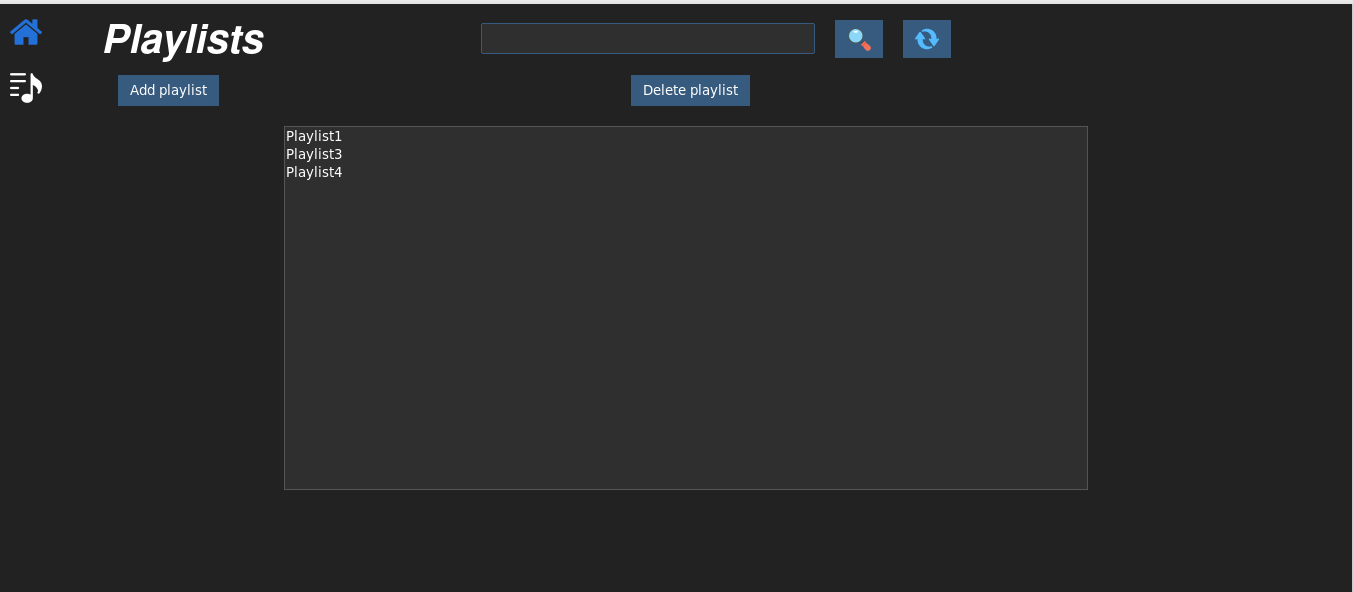
\includegraphics[width=1.0\textwidth]{quanlyplaylist.PNG}
    \caption{Quản Lý Playlist}
    \label{fig:example_image}
\end{figure}

\begin{figure}[H]
    \centering
    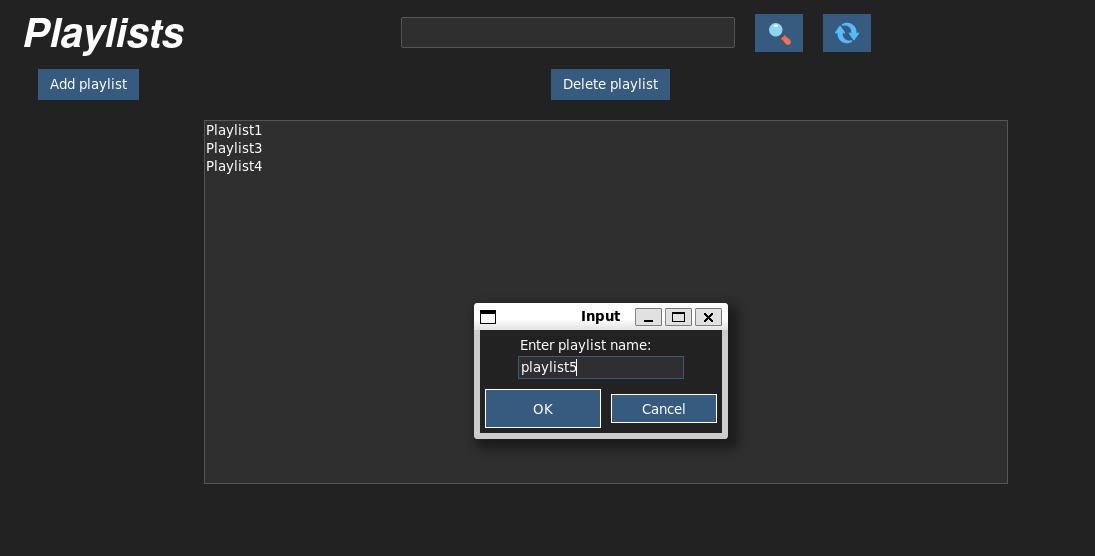
\includegraphics[width=1.0\textwidth]{addplaylist.PNG}
    \caption{Tạo Playlist}
    \label{fig:example_image}
\end{figure}

\begin{figure}[H]
    \centering
    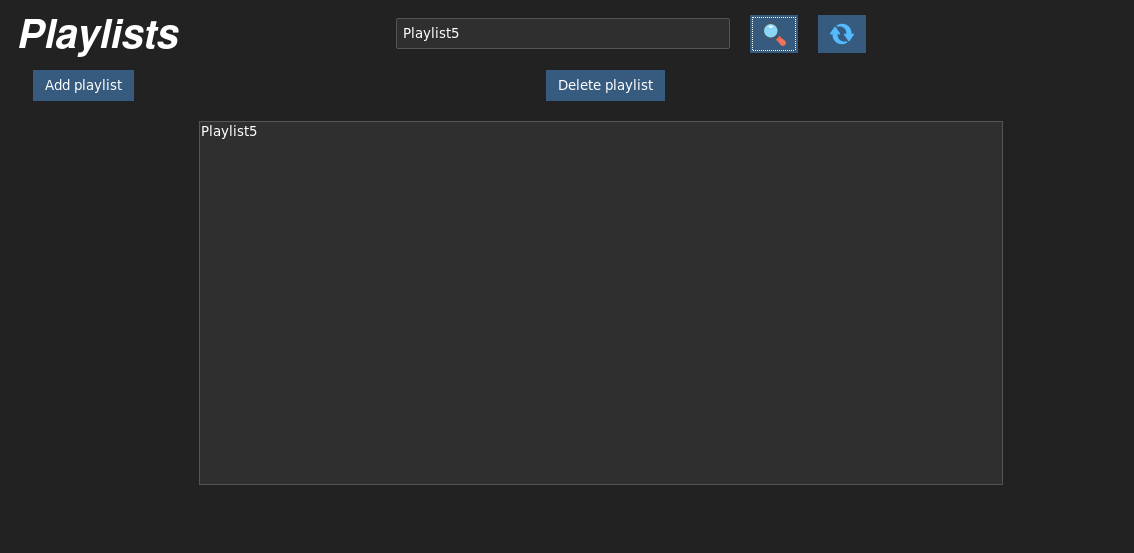
\includegraphics[width=1.0\textwidth]{searchplaylist.PNG}
    \caption{Tìm kiếm Playlist}
    \label{fig:example_image}
\end{figure}

\begin{figure}[H]
    \centering
    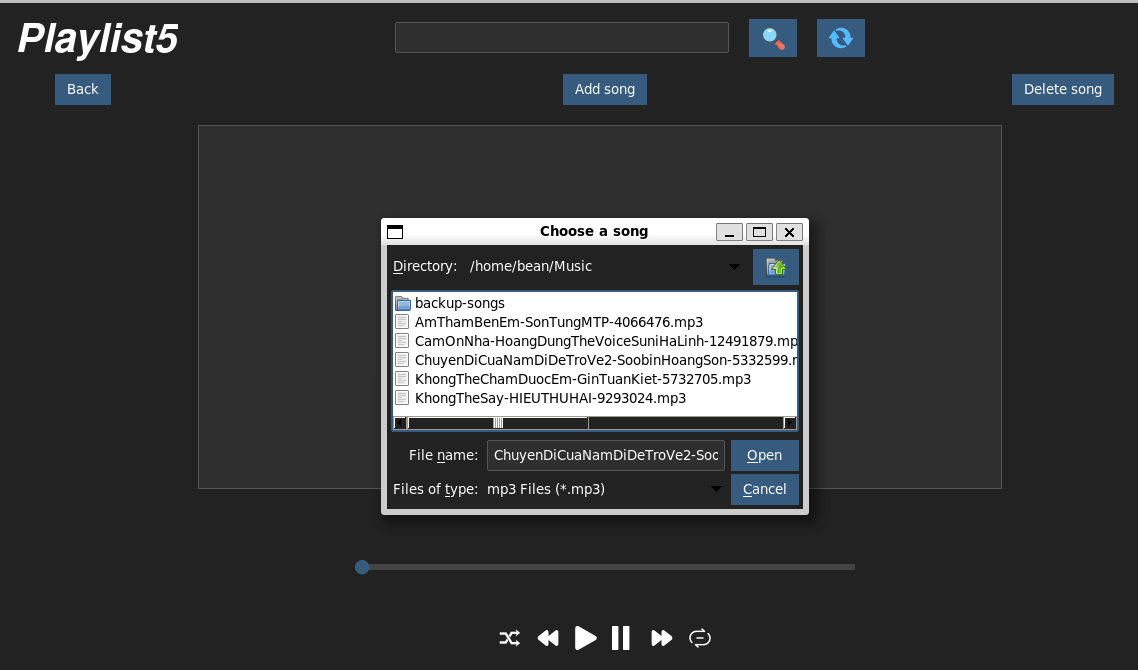
\includegraphics[width=1.0\textwidth]{addsongtoplaylist.PNG}
    \caption{Thêm Bài Hát Vào Playlist}
    \label{fig:example_image}
\end{figure}

\begin{figure}[H]
    \centering
    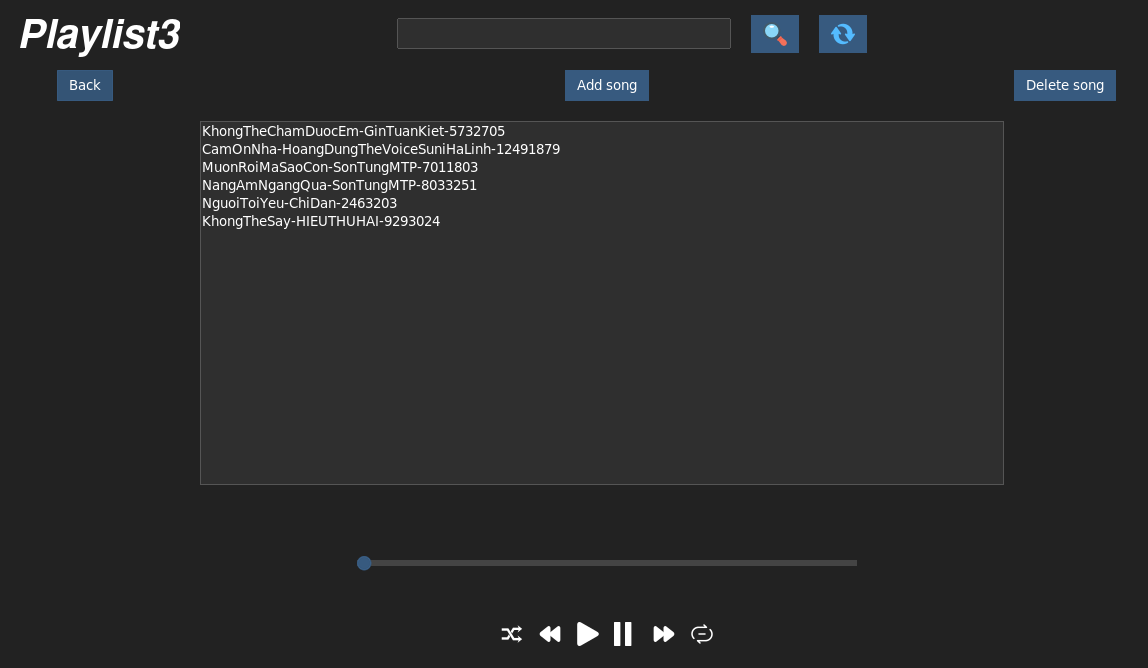
\includegraphics[width=1.0\textwidth]{songsinplaylist.PNG}
    \caption{Danh sách các bài hát trong 1 playlist bất kỳ}
    \label{fig:example_image}
\end{figure}

\begin{figure}[H]
    \centering
    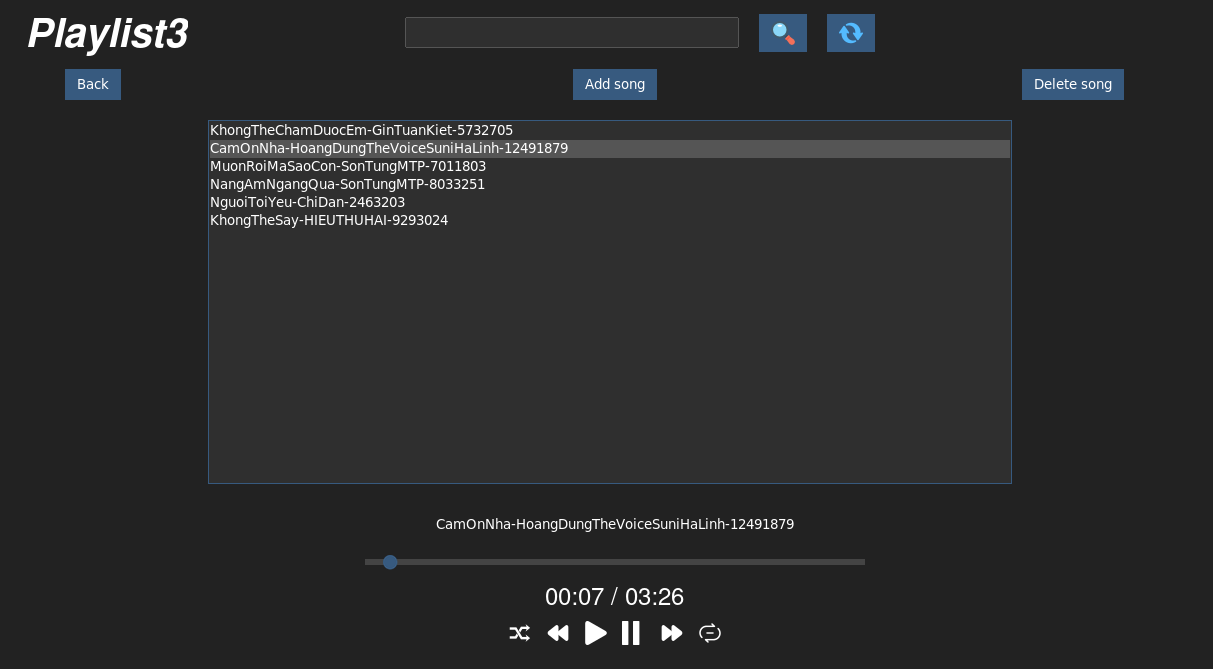
\includegraphics[width=1.0\textwidth]{playsong.PNG}
    \caption{Play 1 Bài Hát}
    \label{fig:example_image}
\end{figure}

\begin{figure}[H]
    \centering
    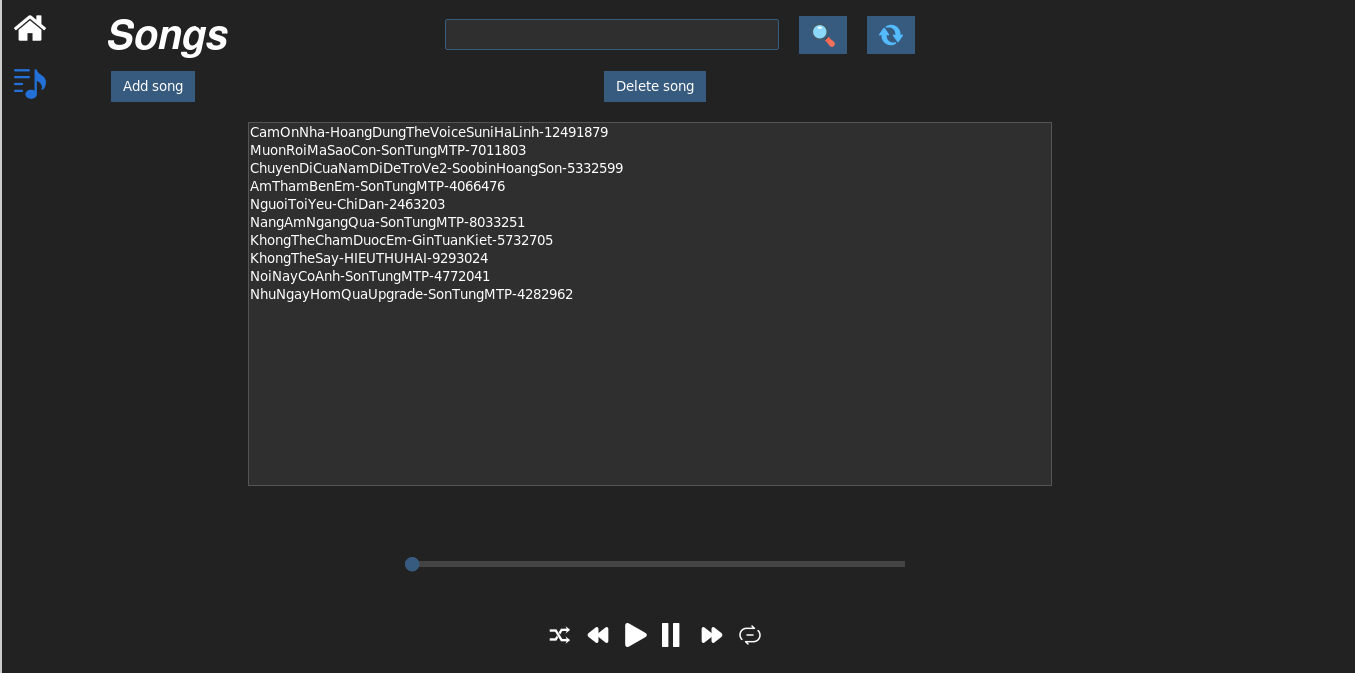
\includegraphics[width=1.0\textwidth]{quanlysong.PNG}
    \caption{Quản Lý Bài Hát}
    \label{fig:example_image}
\end{figure}

\begin{figure}[H]
    \centering
    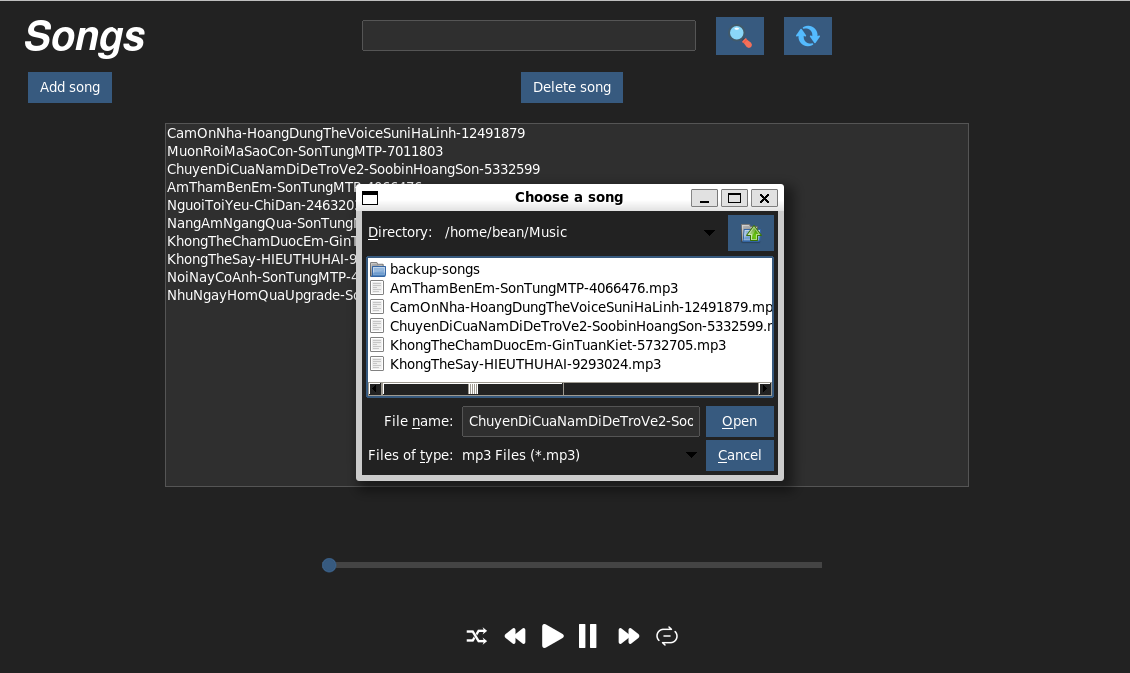
\includegraphics[width=1.0\textwidth]{addsongs.PNG}
    \caption{Thêm Bài Hát}
    \label{fig:example_image}
\end{figure}

\begin{figure}[H]
    \centering
    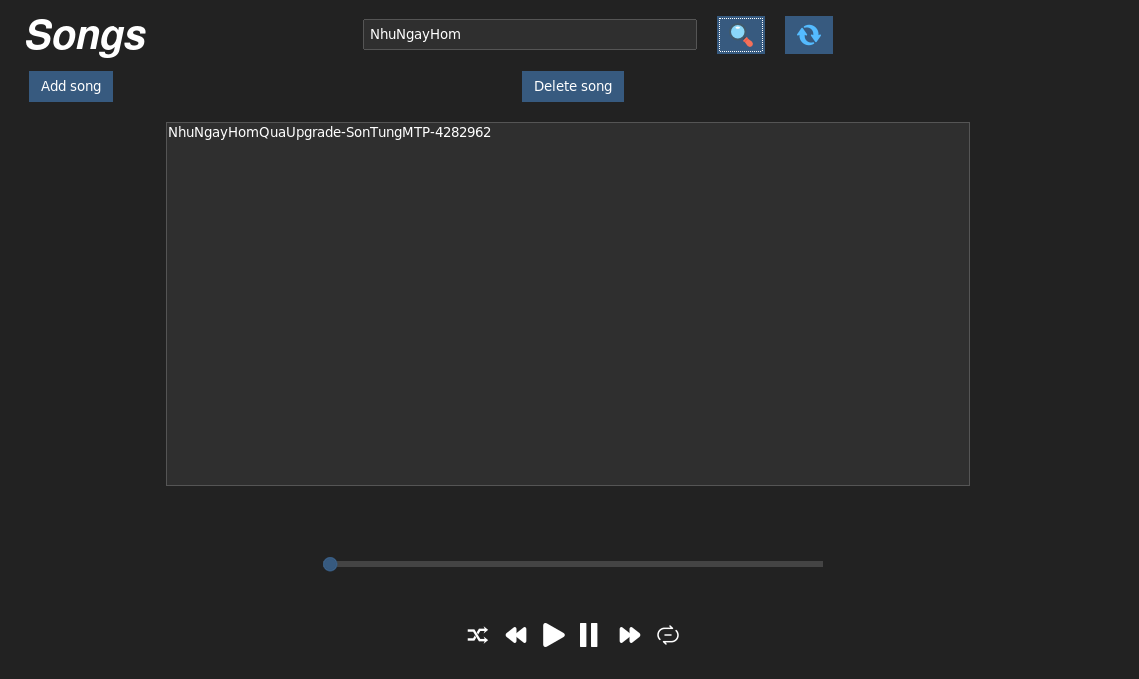
\includegraphics[width=1.0\textwidth]{searchsong.PNG}
    \caption{Tìm Kiếm Bài Hát}
    \label{fig:example_image}
\end{figure}



\section{Cài đặt ứng dụng}
- Sử dụng câu lệnh \textbf{\textit{git clone -b master --single-branch https://github.com/phvu0430/Tkinter-Music-App.git}} để tải ứng dụng về máy. \\
- Sau đó di chuyển vào thư mục \textbf{\textit{Tkinter-Music-App}} và chạy lệnh \textbf{\textit{python3 main.py}} để khởi động ứng dụng.
\newpage
%%%%%%%%%%%%%%%%%%%%%%%%%%%%%%%%%


\newpage
%%%%%%%%%%%%%%%%%%%%%%%%%%%%%%%%%
\begin{thebibliography}{80}

\bibitem{CVX}
John Elder, 
\textbf{\textit{Tkinter Widget Quick Reference Guide}},
\textit{Independently published, 2018}.

\bibitem{CVX}
TTKBootstrap
``\textbf{link: https://ttkbootstrap.readthedocs.io/en/latest/styleguide/}'',
\textit{style guide}, lần truy cập cuối: 25/04/2024.

\bibitem{CVX}
Pygame
``\textbf{link: https://www.pygame.org/docs/ref/music.html/}'',
\textit{pygame.mixer.music}, lần truy cập cuối: 02/05/2024.



\end{thebibliography}
\end{document}

